\documentclass[svgnames,tikz]{standalone}
\usepackage{pgfplots}

\begin{document}
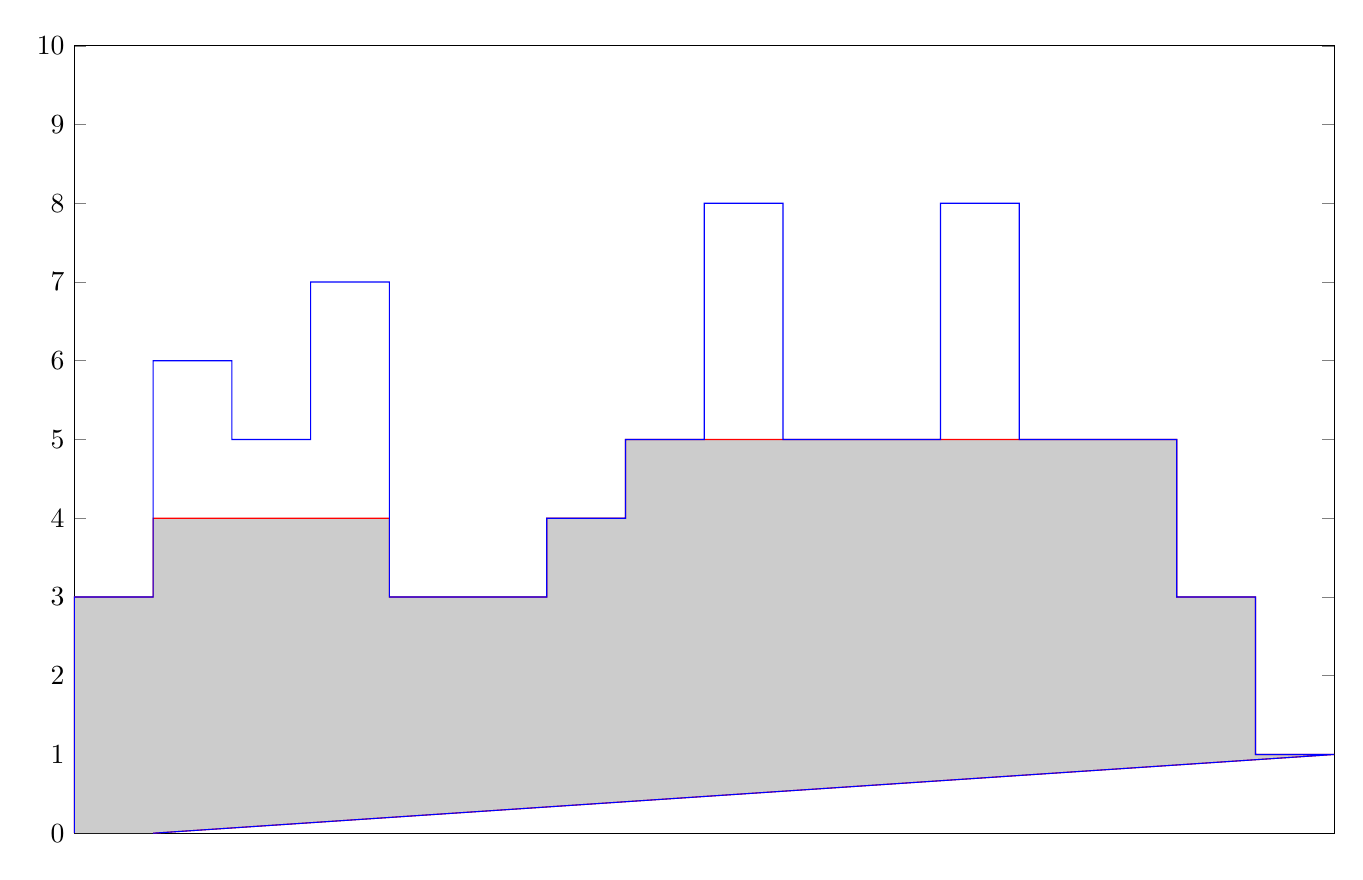
\begin{tikzpicture}[yscale=1]

\def\signalA{3,6,5,7,3,3,4,5,8,5,5,8,5,5,3,1}
\def\signalB{3,4,4,4,3,3,4,5,5,5,5,5,5,5,3,1}

\begin{axis}[
  x=1cm,y=1cm,
  xmin=0,xmax=16,
  ymin=0,ymax=10,
  xtick={\empty},ytick={},
]
\end{axis}


\draw[fill=gray!40,draw=red] (0,0) foreach[count=\x] \y in \signalB { |- (\x,\y) } -- (\x,0);
\draw[blue] (0,0) foreach[count=\x] \y in \signalA { |- (\x,\y) } -- (\x,0);
\end{tikzpicture}
\end{document}
